\documentclass[a4paper,twocolumn,12pt]{article}

\usepackage[margin=0.5in]{geometry}

\usepackage[T2A]{fontenc}
\usepackage[utf8]{inputenc}
\usepackage[russian, english]{babel}

\usepackage{amsmath,amsthm,amssymb}
\usepackage{mathtext}

\usepackage{graphicx}
\usepackage{float}
\usepackage{wrapfig}
\usepackage{caption}
\captionsetup[figure]{name=Рис.} 


\newcommand{\scalar}[2]
{
  \left \langle #1,#2 \right \rangle
}

\newcounter{stage_counter}
\setcounter{stage_counter}{1}

\newenvironment{stage}[1]
{
\begin{center}  
  
  \texttt{\Roman{stage_counter}. #1}      
  
  \addtocounter{stage_counter}{1}
\end{center}  
}{}

\begin{document}

  \begin{stage}{Постановка задачи}
    \[ J(x) = \scalar{a}{x}^4 + 2\|x-b\|^2 \rightarrow \inf, \ x \in \mathbb{R}^5 ,\]
    \[a = (\frac{1}{2}, \frac{1}{4},-\frac{1}{4}, \frac{1}{4}, \frac{3}{4}), b =(2, 4, 3, 3, 0)\]
  \end{stage}
  
  \begin{stage}{Аналитическое решение}
    \[ \scalar{a}{b} = 2, \|a\|^2=1, \|b\|^2=38 \]
    \[ J(x) \ge 0 \Rightarrow \inf \ge 0 > - \infty \] 
    \[ J^{\prime}(x) = 3\scalar{a}{x}^{3}a + 4(x-b) \]
    \[ J^{\prime\prime}(x)h = 12\scalar{a}{x}^{2}\scalar{a}{h}a + 4h 
    \Rightarrow \] 
    \[ \Rightarrow \scalar{J(x)^{\prime\prime}h}{h} \ge 4\|h\|^2 \] 
    \par Значит \(J(x)\) - сильно выпуклая. \\
    \par Так как задача без ограничений, то вариационное неравенство переходит
    в равенство \(\Rightarrow J^\prime(x)=\theta \). 
    Найдем отсюда \(x = \alpha a +\beta b + \gamma c,\) где \( c \perp a,b\):
    \[ 4\scalar{a}{\alpha a +\beta b + \gamma c} + 4(\alpha a +(\beta-1) b + \gamma c) = \theta \Rightarrow\]
    \[ \Rightarrow ((\alpha+2\beta)^3+\alpha)a +(\beta-1)b +\gamma c = \theta \]
    \par Так как \(a, b, c\) - линейно независимы, то коэффициенты при них
    равны нулю, в частности, \(\gamma = 0\) и систему: 
    \[
      \begin{cases}
        \beta = 1\\
        (\alpha+2)^3+\alpha = 0
      \end{cases}
    \Rightarrow 
      \begin{cases}
        \beta = 1\\
        \alpha = -1
      \end{cases}
    \]
    \par По критерию оптимальности \(-a+b\) является точкой глобального минимума. 
    Так как \(J(x)\) -- сильно выпуклая, то точка минимума единственная. 
    \begin{center}
      Ответ: 
      \(J_*=3,\ x_*=-a+b\)
    \end{center}  
  
  \end{stage}

  \begin{stage}{Метод сопряженных градиентов}
    
    Приближение в данном методе строится следующим образом: 
    \[ x_{k+1} = x_k + \alpha_k d_k\]
    \[ d_{k+1} = -f^{\prime}(x_k) + \beta_k d_k, \ d_1 = -f^{\prime}(x_1) \]
    
    Тут настраиваемыми параметрами являются: \(\alpha_k\) и \(\beta_k\).
    
    Будем рассматривать следующие способы выбора \(\beta_k\): 
    
    1) Дай, Юань (1999 г.)
    \[\beta_{k}^{DY} = \frac{\|f^{\prime}(x_{k+1})\|^2}{\scalar{d_k}{y_k}} \]
    
    2) Хагер, Жанг (2005 г.)
    \[ \beta_{k}^{HZ} = \scalar{y_k-2d_k\frac{\|y_{k})\|^2}{\scalar{d_k}{y_k}}}{\frac{f^{\prime}(x_{k+1})}{\scalar{d_k}{y_k}}} \] 
    
    Также кроме константного выбора \(\alpha_k\) будем еще использовать 
    правило Армихо и искать по следующему алгоритму: \\
    \(\alpha_k \leftarrow 2*\alpha_{k-1}\) \\
    \( while \ f(x_k + \alpha_k d_k) > c*\alpha_k*\scalar{f^{\prime}(x_{k})}{d_k} \ do \)
    
    \( \alpha_k \leftarrow \cfrac{\alpha_k}{2} \) \\
    \( end \ while \) \\
    где \(\alpha_0, \ c \) - это гиперпараметры.
  \end{stage}
  
  \begin{stage}{Исследование сходимости от выбора методов.}
    
    Выберем 50 произвольных точек отложенных от \(-a+b\) и посмотрим зависимость расстояния точек от шага.
    
    (стр.2) Ниже можно увидеть графики этой зависимости. Condition: conj (conjugate) - означает, что критерием останова является
    \(\|d_k\| \leq \epsilon\), а dist (distance) - \( \|x_k+1-x_k\| = \|\alpha_k d_k\| \leq \epsilon \). Зафиксируем
    \(\epsilon=0.01\); Для Армихо: \(c=0.25, \alpha_0=1\), а для константного метода: \(\alpha=0.007\).
    На некоторых из них можно увидеть (тяжело, но можно), что процесс при условии dist останавливается раньше как и ожидалось 
    (т.к. \(\alpha_k\) тоже уменьшается). 
    
    (стр.3) В случае Армихо выбирать \(\alpha_0\) большим или маленьким не имеет большого смысла, так как 
    алгоритм сам это сделает, а в случае константного шага, если выбрать \(\alpha=0.5\), то получим, что результат может
    уйти в бесконечность и вовсе выйти за границы численного диапазона всего за 7-8 итераций. Той же проблемной ситуации
    можно добиться от Армихо если положить \(\epsilon = 0.0000001\). 
    
    (стр.3) Можно сравнить методы DY и HZ. Для этого построим графики зависимости среднего кол-ва шагов 
    и стандартного отклонения от расстояния начального вектора до аналитического решения при параметрах 
    \(\epsilon=0.01, c=0.25, \alpha_0=1 \). На каждое расстояние (каждое второе в диапазоне от 5 до 100) 
    было взято 500 начальных позиций. 
    
  \end{stage}
  \newpage

  \onecolumn{
  \begin{figure}[h]
    \centering
    
    \begin{minipage}[h]{0.49\linewidth}
      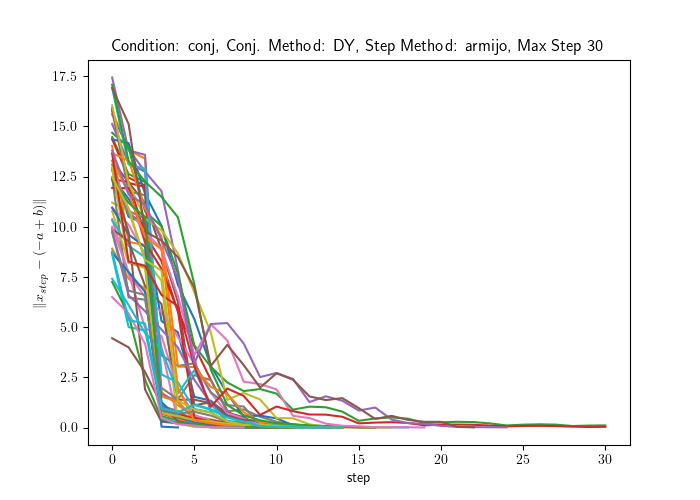
\includegraphics[width=1\linewidth]{./imgs/img1.png}
    \end{minipage}
    \hfill
    \begin{minipage}[h]{0.49\linewidth}
      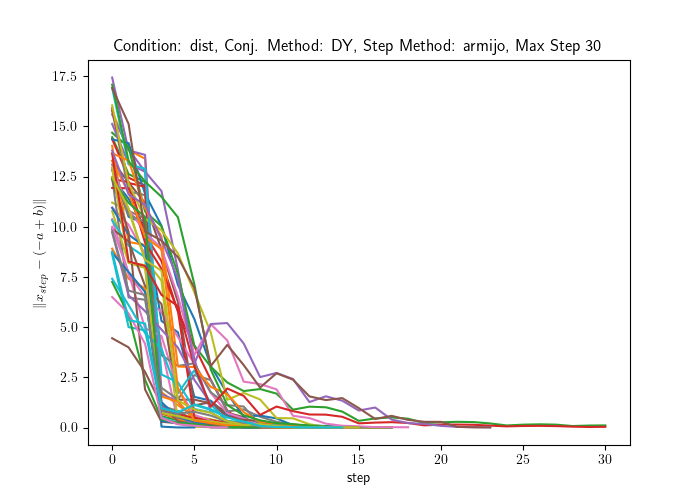
\includegraphics[width=1\linewidth]{./imgs/img2.png}
      \label{fig:mpr}
    \end{minipage}

    \begin{minipage}[h]{0.49\linewidth}
      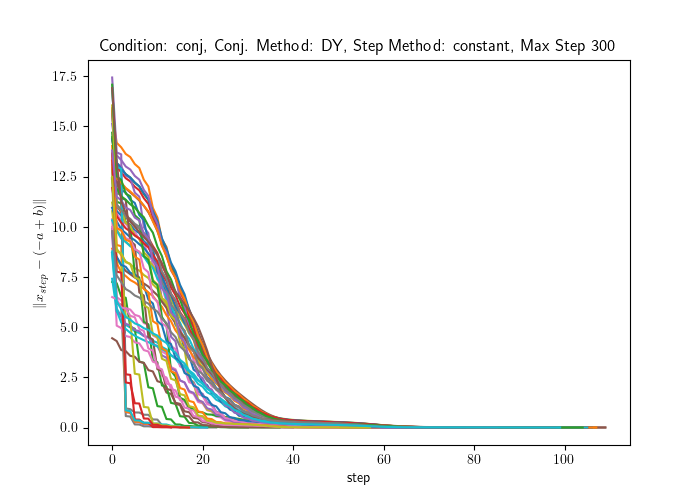
\includegraphics[width=1\linewidth]{./imgs/img3.png}

    \end{minipage}
    \hfill      
    \begin{minipage}[h]{0.49\linewidth}
      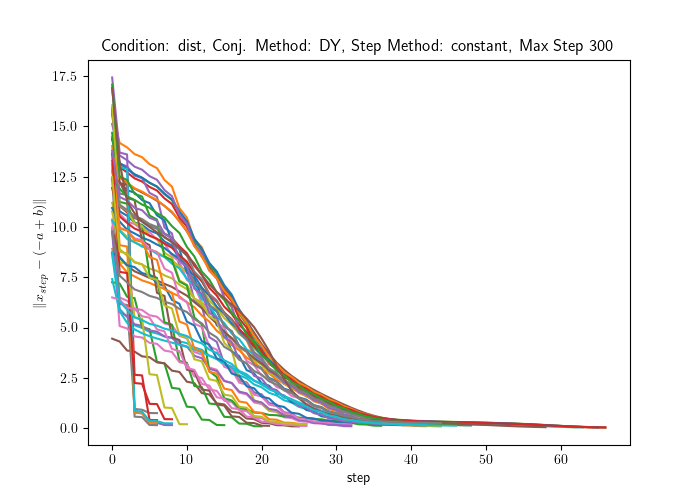
\includegraphics[width=1\linewidth]{./imgs/img4.png}
    \end{minipage}
    
    \begin{minipage}[h]{0.49\linewidth}
      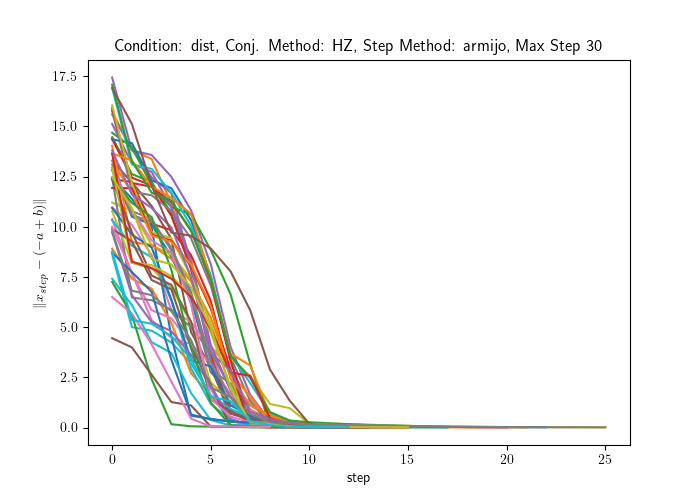
\includegraphics[width=1\linewidth]{./imgs/img5.png}
    \end{minipage}
    \hfill      
    \begin{minipage}[h]{0.49\linewidth}
      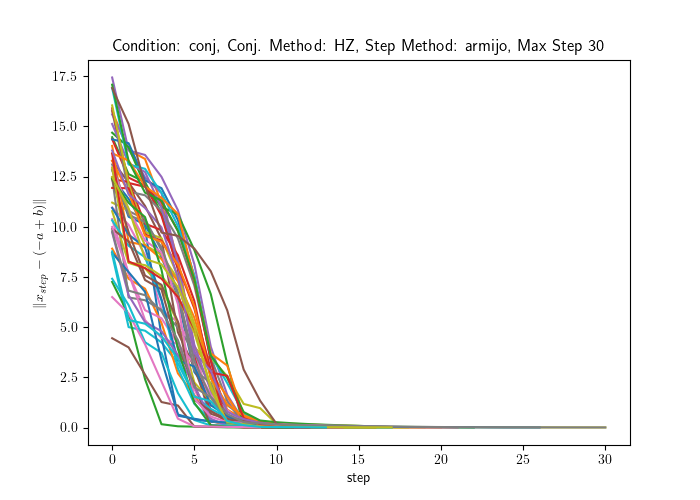
\includegraphics[width=1\linewidth]{./imgs/img6.png}
    \end{minipage}
    
    \begin{minipage}[h]{0.49\linewidth}
      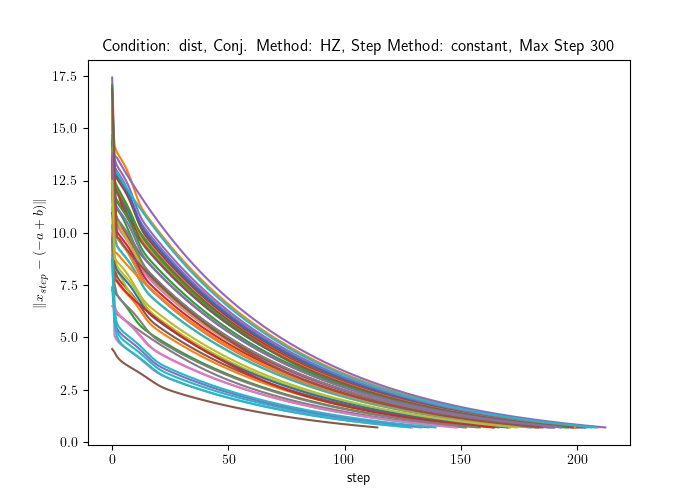
\includegraphics[width=1\linewidth]{./imgs/img7.png}
    \end{minipage}
    \hfill      
    \begin{minipage}[h]{0.49\linewidth}
      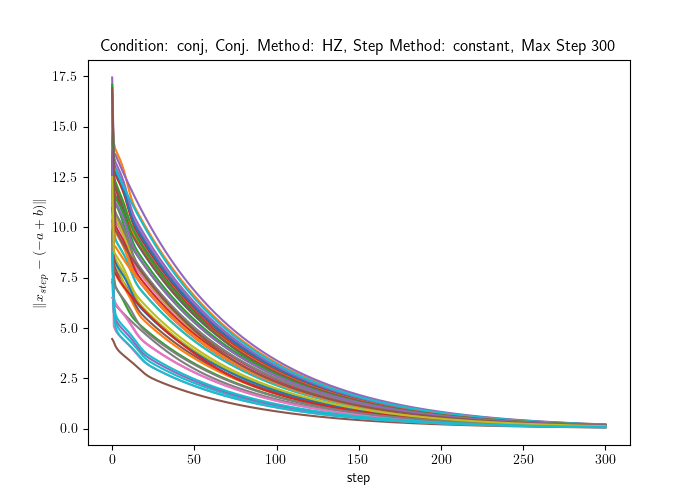
\includegraphics[width=1\linewidth]{./imgs/img8.png}
    \end{minipage}
  \end{figure}

  }

  \newpage
  \onecolumn{
    \centering
    \begin{figure}[h]
      \begin{minipage}[h]{0.49\linewidth}
        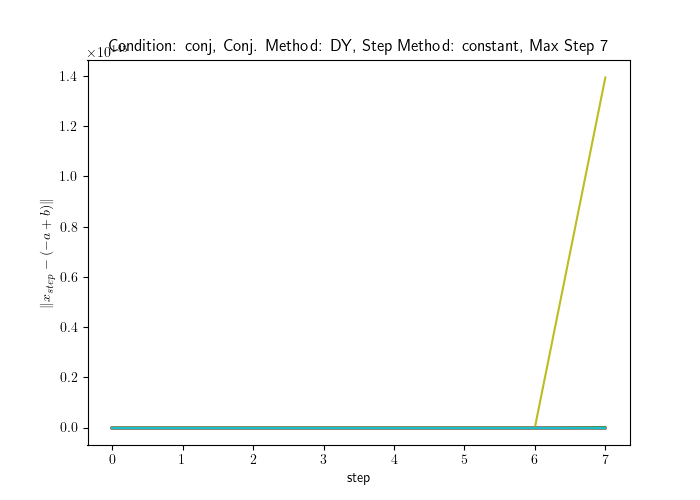
\includegraphics[width=1\linewidth]{./imgs/img9.png}
      \end{minipage}
      \hfill
      \begin{minipage}[h]{0.49\linewidth}
        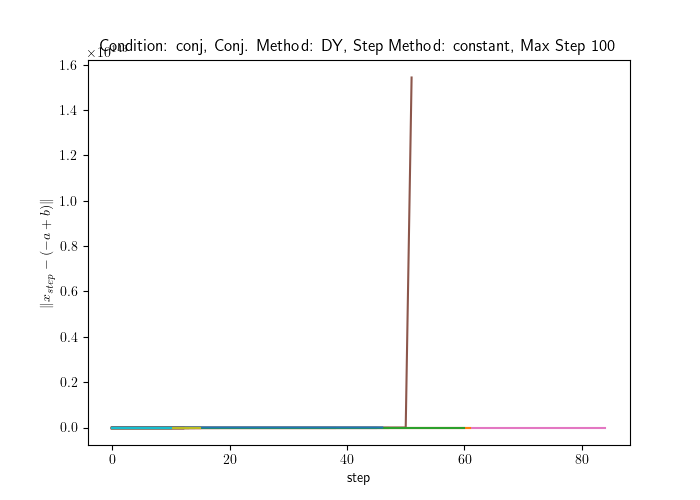
\includegraphics[width=1\linewidth]{./imgs/img10.png}
      \end{minipage}
      
      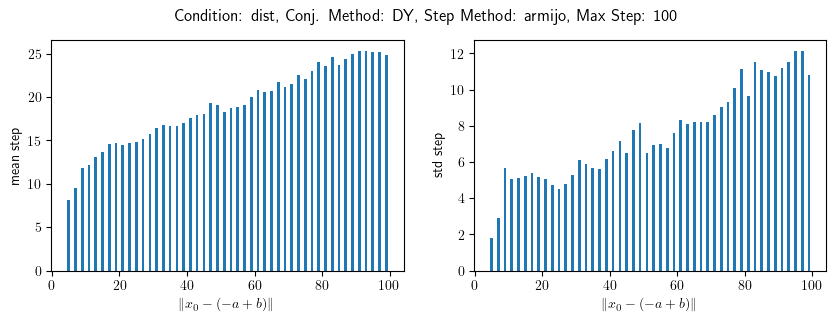
\includegraphics[width=1\linewidth]{./imgs/img11.png}
      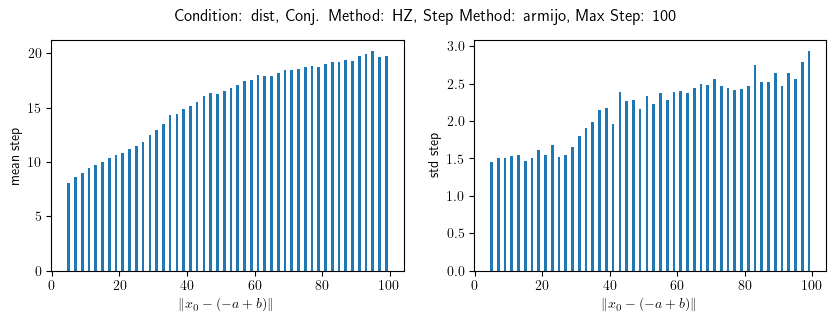
\includegraphics[width=1\linewidth]{./imgs/img12.png}
      
    \end{figure}

  }
  
  \begin{stage}{Вывод}
    Хоть условие Армихо не является "самым-самым" известным сегодня, но показал себя лучше
    чем константный метод (конкретно при заданных параметрах и задаче). Выбор \(\beta^{HZ}\) более здесь
    предпочтителен, так как выигрывает немного в скорости, но что важнее, ведет себя более стабильно
    (это видно на графике стандартного отклонения).    
  \end{stage}
  
\end{document}






